% Capybara Shoot'em Up - User Manual
% Compile with: pdflatex USER_MANUAL.tex

\documentclass[11pt,a4paper]{article}

% Packages
\usepackage[utf8]{inputenc}
\usepackage[margin=1in]{geometry}
\usepackage{graphicx}
\usepackage{xcolor}
\usepackage{colortbl}
\usepackage{tikz}
\usetikzlibrary{shapes.geometric, arrows.meta, positioning, shadows}
\usepackage{tcolorbox}
\usepackage{enumitem}
\usepackage{tabularx}
\usepackage{booktabs}
\usepackage{fancyhdr}
\usepackage{hyperref}
\usepackage{fontawesome5}
\usepackage{multicol}

% Colors
\definecolor{primarycolor}{RGB}{41,128,185}
\definecolor{secondarycolor}{RGB}{52,152,219}
\definecolor{warningcolor}{RGB}{231,76,60}
\definecolor{successcolor}{RGB}{46,204,113}
\definecolor{infocolor}{RGB}{241,196,15}
\definecolor{darkgray}{RGB}{52,73,94}

% Custom box styles
\tcbset{
    mybox/.style={
        colback=primarycolor!5,
        colframe=primarycolor,
        boxrule=1pt,
        arc=3pt,
        left=5pt,
        right=5pt,
        top=5pt,
        bottom=5pt
    }
}

% Header/Footer
\pagestyle{fancy}
\fancyhf{}
\fancyhead[L]{\textcolor{primarycolor}{\textbf{Capybara Shoot'em Up}}}
\fancyhead[R]{\textcolor{darkgray}{User Manual}}
\fancyfoot[C]{\thepage}

% Title page settings
\title{
    \Huge\textbf{\textcolor{primarycolor}{Capybara Shoot'em Up}}\\
    \vspace{0.5cm}
    \Large\textcolor{darkgray}{User Manual \& Strategy Guide}\\
    \vspace{0.3cm}
    \large\textit{Music-Reactive Space Combat}
}

\author{Version 0.9}
\date{\today}

\begin{document}

% Title Page
\maketitle
\thispagestyle{empty}

\begin{center}

\begin{tikzpicture}
    % Spaceship icon
    \fill[primarycolor] (0,0) -- (0.5,1.5) -- (0,2.5) -- (-0.5,1.5) -- cycle;
    \fill[secondarycolor] (-0.3,0.5) -- (0.3,0.5) -- (0.2,1.5) -- (-0.2,1.5) -- cycle;
    \fill[warningcolor] (-0.1,0.3) circle (0.15);
    \fill[warningcolor] (0.1,0.3) circle (0.15);
\end{tikzpicture}

\vspace{1cm}

\Large\textit{Navigate through waves of enemies in this\\
music-synchronized shoot'em up adventure!}
\end{center}

\vfill

\begin{tcolorbox}[colback=infocolor!10, colframe=infocolor, title=\textbf{Quick Start}]
\begin{enumerate}[leftmargin=*]
    \item Build the game: \texttt{make}
    \item Run: \texttt{./bin/shootemup}
    \item Use \textbf{WASD} or \textbf{Arrow Keys} to move
    \item Press \textbf{Space} to shoot
    \item Press \textbf{P} to pause
\end{enumerate}
\end{tcolorbox}

\newpage

% Table of Contents
\tableofcontents
\newpage

%===========================================
\section{Introduction}
%===========================================

\subsection{Welcome}

Welcome to \textbf{Capybara Shoot'em Up}, a thrilling music-reactive space combat game where the intensity of gameplay synchronizes with bass patterns in the soundtrack. Face 10 unique enemy types, master 6 weapon modes, and survive through 9 challenging phases!

\subsection{Game Features}

\begin{itemize}[leftmargin=*]
    \item \textbf{\faMusic~Music-Reactive Gameplay}: Enemy waves spawn based on bass patterns
    \item \textbf{\faRocket~10 Unique Enemy Types}: Each with distinct behaviors and attack patterns
    \item \textbf{\faCrosshairs~6 Weapon Modes}: Single, Double, Spread, Rapid, Dual, and Charge
    \item \textbf{\faStar~4 Powerup Types}: Energy, Shield, Hull, and Weapon upgrades
    \item \textbf{\faBolt~Energy Mode System}: Switch between Offensive and Defensive modes
    \item \textbf{\faSkull~Epic Boss Battles}: Face challenging boss encounters
    \item \textbf{\faChartLine~Progressive Difficulty}: 9 phases of increasing challenge
\end{itemize}

\subsection{System Requirements}

\begin{tcolorbox}[mybox]
\textbf{Minimum Requirements:}
\begin{itemize}[nosep]
    \item \textbf{OS}: macOS 10.14+, Linux (Ubuntu 20.04+), Windows 10+
    \item \textbf{Processor}: 2.0 GHz dual-core
    \item \textbf{Memory}: 2 GB RAM
    \item \textbf{Graphics}: OpenGL 3.3 compatible
    \item \textbf{Storage}: 50 MB available space
    \item \textbf{Audio}: BASS audio library (for music-reactive features)
\end{itemize}
\end{tcolorbox}

%===========================================
\section{Installation}
%===========================================

\subsection{Prerequisites}

\subsubsection{macOS}
\begin{verbatim}
# Install Homebrew
/bin/bash -c "$(curl -fsSL https://raw.githubusercontent.com/
    Homebrew/install/HEAD/install.sh)"

# Install Raylib
brew install raylib

# Install build tools
brew install gcc make pkg-config
\end{verbatim}

\subsubsection{Linux (Ubuntu/Debian)}
\begin{verbatim}
sudo apt update
sudo apt install libraylib-dev build-essential pkg-config
\end{verbatim}

\subsection{Building the Game}

\begin{enumerate}[leftmargin=*]
    \item \textbf{Download or clone the repository}
    \item \textbf{Navigate to the project directory:}
    \begin{verbatim}
    cd capybara-project
    \end{verbatim}
    \item \textbf{Build the game:}
    \begin{verbatim}
    make
    \end{verbatim}
    \item \textbf{Run the game:}
    \begin{verbatim}
    ./bin/shootemup
    \end{verbatim}
\end{enumerate}

\begin{tcolorbox}[colback=successcolor!10, colframe=successcolor, title=\faCheck~Success!]
If the build completes without errors, you'll see the executable in \texttt{bin/shootemup}. You're ready to play!
\end{tcolorbox}

%===========================================
\section{Controls}
%===========================================

\subsection{Basic Controls}

\begin{table}[h]
\centering
\begin{tabularx}{\textwidth}{|l|X|}
\hline
\rowcolor{primarycolor!20}
\textbf{Key} & \textbf{Action} \\
\hline
\textbf{W} / \faArrowUp & Move up \\
\hline
\textbf{S} / \faArrowDown & Move down \\
\hline
\textbf{A} / \faArrowLeft & Move left \\
\hline
\textbf{D} / \faArrowRight & Move right \\
\hline
\textbf{Space} & Shoot \\
\hline
\textbf{P} & Pause/Unpause \\
\hline
\textbf{ESC} & Quit game \\
\hline
\end{tabularx}
\caption{Basic Movement and Combat Controls}
\end{table}

\subsection{Advanced Controls}

\begin{table}[h]
\centering
\begin{tabularx}{\textwidth}{|l|X|}
\hline
\rowcolor{primarycolor!20}
\textbf{Key} & \textbf{Action} \\
\hline
\textbf{1-6} & Select specific weapon mode (1=Single, 2=Spread, 3=Triple, 4=Burst, 5=Rapid, 6=Dual) \\
\hline
\textbf{R} & Cycle through weapon modes \\
\hline
\textbf{Q} & Toggle Energy Mode (Offensive/Defensive) \\
\hline
\textbf{E} (hold) & Use special ability (Offensive: Devastating Attack, Defensive: Enhanced Shield) \\
\hline
\textbf{Hold Space} & Charge weapon (Charge mode only) \\
\hline
\end{tabularx}
\caption{Advanced Combat Controls}
\end{table}

\begin{tcolorbox}[colback=infocolor!10, colframe=infocolor, title=\faLightbulb~Pro Tip]
Hold Space to fire continuously! The weapon has heat management, so watch your overheat indicator.
\end{tcolorbox}

%===========================================
\section{Heads-Up Display (HUD)}
%===========================================

\subsection{HUD Layout}

The game features a two-tier HUD system:

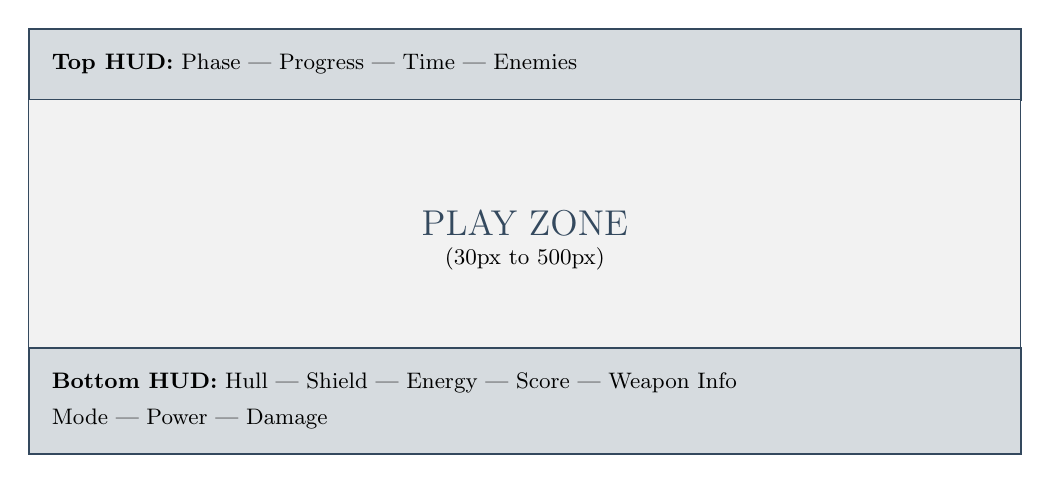
\begin{tikzpicture}[scale=0.9, transform shape]
    % Top HUD
    \draw[fill=darkgray!20, draw=darkgray, thick] (0,5) rectangle (14,6);
    \node[anchor=west] at (0.2,5.5) {\small \textbf{Top HUD:} Phase | Progress | Time | Enemies};
    
    % Play zone
    \draw[fill=black!5, draw=darkgray] (0,1.5) rectangle (14,5);
    \node at (7,3.25) {\Large \textcolor{darkgray}{PLAY ZONE}};
    \node at (7,2.75) {\small (30px to 500px)};
    
    % Bottom HUD
    \draw[fill=darkgray!20, draw=darkgray, thick] (0,0) rectangle (14,1.5);
    \node[anchor=west] at (0.2,1) {\small \textbf{Bottom HUD:} Hull | Shield | Energy | Score | Weapon Info};
    \node[anchor=west] at (0.2,0.5) {\small Mode | Power | Damage};
\end{tikzpicture}

\subsection{Top HUD Elements}

\begin{itemize}[leftmargin=*]
    \item \textbf{Phase Name}: Current wave phase (e.g., "Warm-Up", "Tank Squadron")
    \item \textbf{Progress Bar}: Visual progress through current phase
    \item \textbf{Game Time}: Elapsed time in MM:SS format
    \item \textbf{Enemy Count}: Number of active enemies (red text)
\end{itemize}

\subsection{Bottom HUD Elements}

\subsubsection{Ship Status (Left Side)}

\begin{table}[h]
\centering
\begin{tabularx}{\textwidth}{|l|c|X|}
\hline
\rowcolor{primarycolor!20}
\textbf{Bar} & \textbf{Color} & \textbf{Description} \\
\hline
Hull & \textcolor{red}{\faHeart} Red & Your ship's health. Depletes when shield is down. \\
\hline
Shield & \textcolor{cyan}{\faCircle} Cyan & Regenerating shield. Absorbs damage before hull. \\
\hline
Energy & \textcolor{yellow}{\faBolt} Yellow & Powers special abilities. Regenerates over time. \\
\hline
Mode & \textcolor{orange}{\faCog} Orange/Cyan & Current energy mode with bonus indicator. \\
\hline
\end{tabularx}
\caption{Ship Status Indicators}
\end{table}

\subsubsection{Weapon Info (Center)}

\begin{itemize}[leftmargin=*]
    \item \textbf{Weapon Mode}: Current firing mode (Single, Double, Spread, etc.)
    \item \textbf{Power Level}: Visual sockets showing weapon powerup count (0-3)
    \item \textbf{Damage Per Bullet}: Color-coded damage value with active multipliers
    \item \textbf{Charge Indicator}: Shows charge level for Charge mode
\end{itemize}

\subsubsection{Score (Center-Right)}

Large gold number displaying your current score. Earn points by:
\begin{itemize}[nosep]
    \item Destroying enemies (varies by type)
    \item Collecting powerups (+50 each)
\end{itemize}

%===========================================
\section{Gameplay Mechanics}
%===========================================

\subsection{Ship Systems}

\subsubsection{Hull Integrity}

\begin{tcolorbox}[mybox]
\textbf{Maximum}: 100 HP\\
\textbf{Regeneration}: None (use Hull powerups only)\\
\textbf{Death}: When hull reaches 0 (unless you have weapon powerups)
\end{tcolorbox}

Your hull is your last line of defense. Damage is \textbf{permanent} unless you collect rare Hull powerups. Protect your shield!

\subsubsection{Energy Shield}

\begin{tcolorbox}[mybox]
\textbf{Maximum}: 100 points\\
\textbf{Regeneration}: 2 points/second (after 3-second delay)\\
\textbf{Enhanced Regen}: 4 points/second in Defensive mode (when energy full)
\end{tcolorbox}

Your shield regenerates automatically but requires a brief cooldown after taking damage. Shield powerups provide instant full recovery.

\subsubsection{Energy System}

\begin{tcolorbox}[mybox]
\textbf{Maximum}: 100 points\\
\textbf{Regeneration}: 10 points/second\\
\textbf{Sources}: Natural regen + Energy powerups (+20\%)
\end{tcolorbox}

Energy powers your special abilities. Energy powerups are common drops from most enemies.

\subsection{Energy Modes}

\begin{tikzpicture}[node distance=3cm]
    % Offensive Mode
    \node[draw, rectangle, fill=orange!20, text width=5cm, align=center, thick] (offensive) {
        \textbf{\Large Offensive Mode}\\[0.2cm]
        \textcolor{orange}{\faFire}\\[0.2cm]
        \small
        \textbf{Max Shield: 25}\\[0.1cm]
        \textbf{When Energy Full:}\\
        +100\% Damage\\[0.2cm]
        \textbf{Special (Hold E):}\\
        Devastating Attack
    };
    
    % Defensive Mode
    \node[draw, rectangle, fill=cyan!20, text width=5cm, align=center, thick, right of=offensive] (defensive) {
        \textbf{\Large Defensive Mode}\\[0.2cm]
        \textcolor{cyan}{\faCircle}\\[0.2cm]
        \small
        \textbf{Max Shield: 50}\\[0.1cm]
        \textbf{When Energy Full:}\\
        +100\% Shield Regen\\[0.2cm]
        \textbf{Special (Hold E):}\\
        Enhanced Shield
    };
    
    % Toggle arrow
    \draw[->, very thick, bend left=45] (offensive.north) to node[above] {\textbf{Q}} (defensive.north);
    \draw[->, very thick, bend left=45] (defensive.south) to node[below] {\textbf{Q}} (offensive.south);
\end{tikzpicture}

\begin{tcolorbox}[colback=infocolor!10, colframe=infocolor, title=\faLightbulb~Strategy Tip]
Switch modes based on the situation! Use Offensive when you have high health and want to deal maximum damage. Use Defensive when low on health to boost shield regeneration.
\end{tcolorbox}

\subsection{Weapon Heat Management}

\begin{tikzpicture}[scale=1]
    % Heat bar
    \draw[fill=successcolor!20, draw=black, thick] (0,0) rectangle (10,0.8);
    \draw[fill=successcolor, draw=none] (0,0) rectangle (2,0.8);
    \node at (5,0.4) {\textbf{Heat: 20\%} \textcolor{successcolor}{\faCheckCircle} Safe};
    
    \draw[fill=infocolor!20, draw=black, thick] (0,-1) rectangle (10,0.2);
    \draw[fill=infocolor, draw=none] (0,-1) rectangle (5,0.2);
    \node at (5,-0.4) {\textbf{Heat: 50\%} \textcolor{infocolor}{\faExclamationTriangle} Warning};
    
    \draw[fill=warningcolor!20, draw=black, thick] (0,-2) rectangle (10,-0.8);
    \draw[fill=warningcolor, draw=none] (0,-2) rectangle (9,-0.8);
    \node at (5,-1.4) {\textbf{Heat: 90\%} \textcolor{warningcolor}{\faExclamation} Critical!};
    
    \draw[fill=red!40, draw=black, thick] (0,-3) rectangle (10,-1.8);
    \draw[fill=red, draw=none] (0,-3) rectangle (10,-1.8);
    \node at (5,-2.4) {\textbf{Heat: 100\%} \textcolor{red}{\faTimes} OVERHEATED};
\end{tikzpicture}

\begin{itemize}[leftmargin=*]
    \item \textbf{Heat Generation}: 8\% per shot
    \item \textbf{Cooling Rate}: 30\% per second
    \item \textbf{Overheat Penalty}: 3-second forced cooldown (cannot shoot)
\end{itemize}

\begin{tcolorbox}[colback=warningcolor!10, colframe=warningcolor, title=\faExclamationTriangle~Warning]
Watch your heat! If you overheat, you'll be defenseless for 3 seconds. Learn to fire in bursts!
\end{tcolorbox}

%===========================================
\section{Weapon Systems}
%===========================================

\subsection{Weapon Modes}

\begin{table}[h]
\centering
\small
\begin{tabularx}{\textwidth}{|l|c|c|X|}
\hline
\rowcolor{primarycolor!20}
\textbf{Mode} & \textbf{Key} & \textbf{Bullets} & \textbf{Description} \\
\hline
Single & 1 & 1 & High damage single shot. Best for precision. \\
\hline
Double & 2 & 2 & Two bullets at slight angles. Balanced option. \\
\hline
Spread & 3 & 3 & Wide spread pattern. Great for coverage. \\
\hline
Rapid & 4 & 1 & Single shot, 2× fire rate. High DPS. \\
\hline
Dual & 5 & 2 & Two parallel bullets. Consistent damage. \\
\hline
Charge & 6 & Varies & Hold to charge, release for burst. \\
\hline
\end{tabularx}
\caption{Weapon Modes Comparison}
\end{table}

\subsection{Base Damage Per Bullet}

\begin{table}[h]
\centering
\begin{tabularx}{\textwidth}{|l|c|c|c|}
\hline
\rowcolor{primarycolor!20}
\textbf{Mode} & \textbf{Damage/Bullet} & \textbf{Total Damage} & \textbf{Best For} \\
\hline
Single & 3.0 & 3.0 & Single targets, precision \\
\hline
Double & 1.5 & 3.0 & General purpose \\
\hline
Spread & 1.0 & 3.0 & Multiple targets, area \\
\hline
Rapid & 1.5 & 3.0/sec × 2 & Sustained DPS \\
\hline
Dual & 1.5 & 3.0 & Reliable hits \\
\hline
Charge & 1.0 × bullets & Varies & Burst damage \\
\hline
\end{tabularx}
\caption{Weapon Damage Breakdown}
\end{table}

\subsection{Weapon Powerup Multipliers}

Collect \textcolor{orange}{\faStar} Weapon powerups to increase your damage!

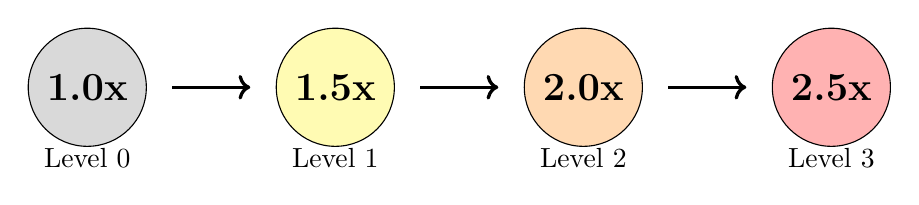
\begin{tikzpicture}[scale=0.9]
    \foreach \x/\mult/\color in {0/1.0x/gray, 3.5/1.5x/yellow, 7/2.0x/orange, 10.5/2.5x/red} {
        \node[circle, draw, fill=\color!30, minimum size=1.5cm] at (\x,0) {\Large \textbf{\mult}};
    }
    \node at (0,-1) {Level 0};
    \node at (3.5,-1) {Level 1};
    \node at (7,-1) {Level 2};
    \node at (10.5,-1) {Level 3};
    
    \draw[->, very thick] (1.2,0) -- (2.3,0);
    \draw[->, very thick] (4.7,0) -- (5.8,0);
    \draw[->, very thick] (8.2,0) -- (9.3,0);
\end{tikzpicture}

\begin{center}
\textbf{Maximum Damage:} Single mode × 2.5x powerup × 2x offensive = \textcolor{red}{\textbf{15.0 damage per bullet!}}
\end{center}

\subsection{Damage Calculation Formula}

\begin{tcolorbox}[mybox]
\centering
\Large
\textbf{Damage Per Bullet} = \\[0.3cm]
Base Damage × Weapon Multiplier × Offensive Bonus\\[0.2cm]
\normalsize
(Offensive Bonus = 2× when energy is FULL in Offensive mode)
\end{tcolorbox}

%===========================================
\section{Powerup System}
%===========================================

\subsection{Powerup Types}

\begin{table}[h]
\centering
\begin{tabularx}{\textwidth}{|l|c|c|X|}
\hline
\rowcolor{primarycolor!20}
\textbf{Type} & \textbf{Visual} & \textbf{Effect} & \textbf{Rarity} \\
\hline
Energy & \textcolor{yellow}{\faLightbulb} Yellow & Restores 20\% energy & Common \\
\hline
Shield & \textcolor{cyan}{\faCircle} Cyan & Fully restores shield & Uncommon \\
\hline
Hull & \textcolor{red}{\faHeart} Red & Repairs 20\% hull & Very Rare \\
\hline
Weapon & \textcolor{orange}{\faStar} Orange & Increases weapon level & Rare \\
\hline
\end{tabularx}
\caption{Powerup Types and Effects}
\end{table}

\subsection{Powerup Behavior}

\begin{itemize}[leftmargin=*]
    \item \textbf{Drift}: Powerups drift left at 25 pixels/second
    \item \textbf{Magnetic Collection}: Attracted to you within 80 pixels
    \item \textbf{Lifetime}: 15 seconds before despawning
    \item \textbf{Fade-Out}: Last 3 seconds show fade effect
    \item \textbf{Score Bonus}: +50 points per powerup collected
\end{itemize}

\begin{tcolorbox}[colback=successcolor!10, colframe=successcolor, title=\faCheck~Collection Tip]
Stay near powerups to trigger magnetic attraction! They'll fly toward you automatically.
\end{tcolorbox}

\subsection{Weapon Powerup Revival System}

\begin{tcolorbox}[colback=infocolor!10, colframe=infocolor, title=\faLightbulb~Extra Lives!]
Each weapon powerup level acts as an \textbf{extra life}! When your hull reaches 0:
\begin{enumerate}[nosep]
    \item One weapon level is consumed
    \item Hull restored to 33\%
    \item Shield restored to 50\%
    \item Golden revival aura appears for 2 seconds
\end{enumerate}

With 3 weapon powerups, you have \textbf{4 total lives}!
\end{tcolorbox}

%===========================================
\section{Enemy Types}
%===========================================

\subsection{Enemy Overview}

The game features 10 unique enemy types, each with distinct behaviors:

\begin{table}[h]
\centering
\small
\begin{tabularx}{\textwidth}{|l|c|c|X|}
\hline
\rowcolor{primarycolor!20}
\textbf{Enemy} & \textbf{Difficulty} & \textbf{Health} & \textbf{Behavior} \\
\hline
Grunt & \faCircle & Low & Basic straight movement \\
\hline
Swarm & \faCircle & Very Low & Small, numerous, fast \\
\hline
Speeder & \faCircle\faCircle & Low & Fast zig-zag movement \\
\hline
Zigzag & \faCircle\faCircle & Medium & Unpredictable patterns \\
\hline
Bomber & \faCircle\faCircle\faCircle & Medium & Area attacks \\
\hline
Tank & \faCircle\faCircle\faCircle & High & Slow, heavy armor, missiles \\
\hline
Shield & \faCircle\faCircle\faCircle & Medium & Rotating shield protection \\
\hline
Ghost & \faCircle\faCircle\faCircle & Medium & Phase in/out ability \\
\hline
Elite & \faCircle\faCircle\faCircle\faCircle & High & Advanced AI \\
\hline
Boss & \faCircle\faCircle\faCircle\faCircle\faCircle & Very High & Complex patterns \\
\hline
\end{tabularx}
\caption{Enemy Types by Difficulty}
\end{table}

\subsection{Enemy Projectiles}

Enemies fire 4 types of projectiles:

\begin{table}[h]
\centering
\begin{tabularx}{\textwidth}{|l|c|X|}
\hline
\rowcolor{primarycolor!20}
\textbf{Type} & \textbf{Speed} & \textbf{Characteristic} \\
\hline
Laser & Fast & Straight line, basic \\
\hline
Plasma & Medium & Slight homing (30\%) \\
\hline
Missile & Medium-Fast & Strong homing (70\%), explosive \\
\hline
Energy Orb & Slow & Wave motion, piercing, explosive \\
\hline
\end{tabularx}
\caption{Enemy Projectile Types}
\end{table}

\begin{tcolorbox}[colback=warningcolor!10, colframe=warningcolor, title=\faExclamationTriangle~Watch Out!]
\textbf{Tank enemies} fire 3 homing missiles in a spread pattern! Multiple Tanks can create overwhelming missile barrages. Prioritize destroying Tanks first!
\end{tcolorbox}

%===========================================
\section{Game Phases}
%===========================================

\subsection{Phase Progression}

The game consists of 9 major phases over approximately 9 minutes:

\begin{table}[h]
\centering
\small
\begin{tabularx}{\textwidth}{|c|l|X|}
\hline
\rowcolor{primarycolor!20}
\textbf{Phase} & \textbf{Name} & \textbf{Description} \\
\hline
1 & Warm-Up & Gentle introduction, no enemies \\
\hline
2 & First Wave & Basic Grunt enemies, no firing \\
\hline
3 & Tank Squadron & Heavy armored Tanks with missiles \\
\hline
4 & Swarm Attack & Numerous small fast enemies \\
\hline
5 & Mixed Assault & Combined enemy types \\
\hline
6 & Elite Squadron & Advanced AI enemies \\
\hline
7 & Zigzag Chaos & Unpredictable movement patterns \\
\hline
8 & Shield Wall & Shielded enemies require timing \\
\hline
9 & Final Challenge & All enemy types, Boss included \\
\hline
\end{tabularx}
\caption{Game Phase Overview}
\end{table}

\subsection{Boss Encounters}

\textbf{Boss Spawn Time}: Approximately 7 minutes (427 seconds)

The Boss features:
\begin{itemize}[nosep]
    \item Massive health pool
    \item Complex attack patterns
    \item Multiple projectile types
    \item 360° radial attacks
    \item Guaranteed powerup drop on defeat
\end{itemize}

%===========================================
\section{Strategy Guide}
%===========================================

\subsection{Beginner Tips}

\begin{enumerate}[leftmargin=*]
    \item \textbf{Use your shield}: Let it regenerate between enemy waves
    \item \textbf{Collect powerups}: Don't miss them! They drift off-screen quickly
    \item \textbf{Watch enemy patterns}: Each type has predictable movement
    \item \textbf{Prioritize threats}: Kill Tanks and Bombers first
    \item \textbf{Save weapon powerups}: They're extra lives!
    \item \textbf{Switch energy modes}: Adapt to the situation
    \item \textbf{Use Spread mode}: Great for beginners due to wide coverage
    \item \textbf{Stay mobile}: Keep moving to avoid enemy fire
\end{enumerate}

\subsection{Advanced Strategies}

\subsubsection{Weapon Mode Selection}

\begin{itemize}[leftmargin=*]
    \item \textbf{Single}: Maximum damage against bosses and tanks
    \item \textbf{Spread}: Best for Swarm enemies and crowd control
    \item \textbf{Rapid}: Consistent DPS against medium enemies
    \item \textbf{Charge}: Burst damage for clearing groups
\end{itemize}

\subsubsection{Energy Mode Tactics}

\begin{tcolorbox}[mybox]
\textbf{Offensive Mode Strategy:}
\begin{itemize}[nosep]
    \item Keep energy full for 2× damage bonus
    \item Use devastating attack to clear dense waves
    \item Best when you have high hull/shield
\end{itemize}

\textbf{Defensive Mode Strategy:}
\begin{itemize}[nosep]
    \item Use when low on health
    \item Enhanced shield ability buys time
    \item 2× shield regen helps recovery
    \item Switch to Offensive once recovered
\end{itemize}
\end{tcolorbox}

\subsubsection{Powerup Prioritization}

\textbf{Priority Order:}
\begin{enumerate}[nosep]
    \item \textcolor{red}{\faHeart} \textbf{Hull} - Only way to restore hull!
    \item \textcolor{orange}{\faStar} \textbf{Weapon} - Extra lives + damage
    \item \textcolor{cyan}{\faCircle} \textbf{Shield} - Instant protection
    \item \textcolor{yellow}{\faLightbulb} \textbf{Energy} - Common, get if convenient
\end{enumerate}

\subsubsection{Boss Fight Strategy}

\begin{enumerate}[leftmargin=*]
    \item \textbf{Stock up before}: Collect powerups from pre-boss waves
    \item \textbf{Use Single mode}: Maximum damage per bullet
    \item \textbf{Stay in Offensive}: Keep energy full for 2× damage
    \item \textbf{Circle strafe}: Move in circles to avoid radial attacks
    \item \textbf{Focus fire}: Don't stop shooting!
    \item \textbf{Save special ability}: Use devastating attack when overwhelmed
\end{enumerate}

\subsection{Survival Tips}

\begin{tcolorbox}[colback=successcolor!10, colframe=successcolor, title=\faHeart~Stay Alive!]
\begin{itemize}[nosep]
    \item \textbf{Dodge first, shoot second}: Survival > damage
    \item \textbf{Use the full play zone}: Don't corner yourself
    \item \textbf{Watch projectile patterns}: Learn to predict
    \item \textbf{Let shield regenerate}: Back off when shield is low
    \item \textbf{Don't waste weapon powerups}: They're your extra lives!
    \item \textbf{Pause when overwhelmed}: Use P to assess the situation
\end{itemize}
\end{tcolorbox}

%===========================================
\section{Scoring System}
%===========================================

\subsection{Points Breakdown}

\begin{table}[h]
\centering
\begin{tabularx}{\textwidth}{|l|c|X|}
\hline
\rowcolor{primarycolor!20}
\textbf{Action} & \textbf{Points} & \textbf{Notes} \\
\hline
Grunt destroyed & ~10 & Basic enemy \\
\hline
Tank destroyed & ~20 & Heavy enemy \\
\hline
Elite destroyed & ~30 & Advanced enemy \\
\hline
Boss destroyed & ~100 & Major achievement \\
\hline
Powerup collected & +50 & Any type \\
\hline
\end{tabularx}
\caption{Scoring System}
\end{table}

\textit{Note: Exact enemy scores vary based on enemy power rating}

%===========================================
\section{Troubleshooting}
%===========================================

\subsection{Common Issues}

\subsubsection{Game Won't Build}

\textbf{Error}: \texttt{raylib.h not found}

\textbf{Solution}:
\begin{verbatim}
# macOS
brew reinstall raylib

# Linux
sudo apt install --reinstall libraylib-dev
\end{verbatim}

\subsubsection{Game Crashes on Start}

\textbf{Possible causes}:
\begin{itemize}[nosep]
    \item Missing audio file: Place music in \texttt{assets/audio/}
    \item BASS library not installed
    \item OpenGL driver issues
\end{itemize}

\subsubsection{Low Frame Rate}

\textbf{Solutions}:
\begin{itemize}[nosep]
    \item Close other applications
    \item Update graphics drivers
    \item Reduce particle effects (future option)
\end{itemize}

\subsubsection{Audio Not Playing}

\textbf{Check}:
\begin{itemize}[nosep]
    \item BASS library installed correctly
    \item Audio file exists in \texttt{assets/audio/}
    \item System audio not muted
\end{itemize}

\subsection{Performance Tips}

\begin{itemize}[leftmargin=*]
    \item Target: \textbf{60 FPS} constant
    \item Close background applications
    \item Ensure adequate system resources
    \item Update to latest version
\end{itemize}

%===========================================
\section{Credits \& Acknowledgments}
%===========================================

\subsection{Development}

\textbf{Capybara Shoot'em Up} is an open-source project built with:

\begin{itemize}[leftmargin=*]
    \item \textbf{Raylib} - Graphics and game framework
    \item \textbf{BASS Audio Library} - Music analysis and playback
    \item \textbf{C99} - Programming language
    \item \textbf{Love and Passion} - From the developer community
\end{itemize}

\subsection{Special Thanks}

Thank you to all contributors, testers, and players who helped make this game possible!

%===========================================
\section{Appendix}
%===========================================

\subsection{Quick Reference Card}

\begin{tcolorbox}[mybox, title=\textbf{Quick Reference}]
\begin{multicols}{2}
\textbf{Movement:}
\begin{itemize}[nosep]
    \item WASD / Arrows
\end{itemize}

\textbf{Combat:}
\begin{itemize}[nosep]
    \item Space: Shoot
    \item 1-6: Select specific weapon mode
    \item R: Cycle weapon modes
    \item Q: Toggle energy mode
    \item E: Special ability
\end{itemize}

\textbf{System:}
\begin{itemize}[nosep]
    \item P: Pause
    \item ESC: Quit
\end{itemize}

\columnbreak

\textbf{Powerups:}
\begin{itemize}[nosep]
    \item \textcolor{yellow}{Yellow}: Energy
    \item \textcolor{cyan}{Cyan}: Shield
    \item \textcolor{red}{Red}: Hull
    \item \textcolor{orange}{Orange}: Weapon
\end{itemize}

\textbf{Strategy:}
\begin{itemize}[nosep]
    \item Dodge > Shoot
    \item Collect everything
    \item Watch your heat
    \item Use full screen
\end{itemize}
\end{multicols}
\end{tcolorbox}

\subsection{Keyboard Layout}

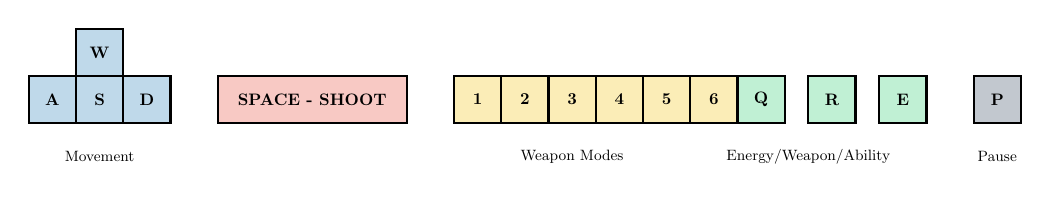
\begin{tikzpicture}[scale=0.6, transform shape]
    % WASD cluster
    \draw[fill=primarycolor!30, thick] (0,1) rectangle (1,2) node[pos=.5] {\textbf{W}};
    \draw[fill=primarycolor!30, thick] (-1,0) rectangle (0,1) node[pos=.5] {\textbf{A}};
    \draw[fill=primarycolor!30, thick] (0,0) rectangle (1,1) node[pos=.5] {\textbf{S}};
    \draw[fill=primarycolor!30, thick] (1,0) rectangle (2,1) node[pos=.5] {\textbf{D}};
    
    \node at (0.5,-0.7) {\small Movement};
    
    % Space bar
    \draw[fill=warningcolor!30, thick] (3,0) rectangle (7,1) node[pos=.5] {\textbf{SPACE - SHOOT}};
    
    % Numbers
    \foreach \x/\n in {8/1, 9/2, 10/3, 11/4, 12/5, 13/6} {
        \draw[fill=infocolor!30, thick] (\x,0) rectangle (\x+1,1) node[pos=.5] {\textbf{\n}};
    }
    \node at (10.5,-0.7) {\small Weapon Modes};
    
    % Q, R and E
    \draw[fill=successcolor!30, thick] (14,0) rectangle (15,1) node[pos=.5] {\textbf{Q}};
    \draw[fill=successcolor!30, thick] (15.5,0) rectangle (16.5,1) node[pos=.5] {\textbf{R}};
    \draw[fill=successcolor!30, thick] (17,0) rectangle (18,1) node[pos=.5] {\textbf{E}};
    
    \node at (15.5,-0.7) {\small Energy/Weapon/Ability};
    
    % P
    \draw[fill=darkgray!30, thick] (19,0) rectangle (20,1) node[pos=.5] {\textbf{P}};
    \node at (19.5,-0.7) {\small Pause};
\end{tikzpicture}

\subsection{Version Information}

\begin{itemize}[leftmargin=*]
    \item \textbf{Version}: 0.9 (Development Build)
    \item \textbf{Manual Version}: 1.0
    \item \textbf{Last Updated}: \today
\end{itemize}

%===========================================

\vfill

\begin{center}
\Large
\textbf{Good Luck, Pilot!}\\
\vspace{0.5cm}
\normalsize
May your aim be true and your powerups plentiful!\\
\vspace{0.5cm}
\textcolor{primarycolor}{\faRocket~\faRocket~\faRocket}
\end{center}

\end{document}
